\section{Part A -- Finite Difference Methods}
\subsection{Explicit Finite Difference Solutions}
\subsubsection{AR and PE plots} \label{fdm-explicit-ARPE}
The analytical amplification factor and phase shift of the equation \ref{eq:1} are
\begin{subequations}
  \begin{equation}
    \label{eq:3a}
    \Phi_n^{anal} = e^{-4\pi^2 \mathcal{D} (\frac{\Delta x}{\Lambda_n})^2} e^{-2\pi \mathcal{U} \frac{\Delta x}{\Lambda_n}}
  \end{equation}
  \begin{equation}
    \label{eq:3b}
    \Delta \Theta_n^{anal} = -2\pi \mathcal{U}\frac{\Delta x}{\Lambda_n}
  \end{equation}
\end{subequations}
where $\mathcal{D}=\frac{D\Delta t}{\Delta x^2}$ and $\mathcal{U}=\frac{U\Delta t}{\Delta x}$.

The numerical solutions of the amplification factor and phase shift of the upstream method are
\begin{subequations}
  \begin{equation}
    \label{eq:4a}
    \Phi_n^{fdm,explicit,up} = 1-(2\mathcal{D}+\mathcal{U})(1-\cos{2\pi \frac{\Delta x}{\Lambda_n}}) - i\mathcal{U}\sin{2\pi \frac{\Delta x}{\Lambda_n}}
  \end{equation}
  \begin{equation}
    \label{eq:4b}
    \Delta \Theta_n^{fdm,explicit,up} = \sin^{-1}[\frac{-\mathcal{U}\sin{2\pi\frac{\Delta x}{\Lambda_n}}}{|\Phi_n^{fdm,up}|}]
  \end{equation}
\end{subequations}

The numberical solutions of the amplification factor and phase shift of the central method are
\begin{subequations}
  \begin{equation}
    \label{eq:5a}
    \Phi_n^{fdm,explicit,central} = 1-2\mathcal{D}(1-\cos{2\pi \frac{\Delta x}{\Lambda_n}}) - i\mathcal{U}\sin{2\pi \frac{\Delta x}{\Lambda_n}}
  \end{equation}
  \begin{equation}
    \label{eq:5b}
    \Delta \Theta_n^{fdm,explicit,central} = \sin^{-1}[\frac{-\mathcal{U}\sin{2\pi\frac{\Delta x}{\Lambda_n}}}{|\Phi_n^{fdm,explicit,central}|}]
  \end{equation}
\end{subequations}

Also, as we know that the amplification ratio $AR = (\frac{|\Phi_n^{num}|}{|\Phi_n^{anal}|})^{Nn}$ and the phase error $PE = -2\pi-Nn\Delta \Theta_n^{num}$, the amplification ratios and the phase errors of the two methods can be obtained as follows.
\begin{subequations}
  \begin{equation}
    \label{eq:6a}
    AR_{fdm,explicit,i} = (\frac{|\Phi_n^{fdm,explicit,i}|}{|\Phi_n^{anal}|})^{Nn}
  \end{equation}
  \begin{equation}
    \label{eq:6b}
    PE_{fdm,explicit,i} = -2\pi-Nn\Delta \Theta_n^{fdm,explicit,i}
  \end{equation}
\end{subequations}
where $i=up,central$.

\paragraph{Settings}\label{partA-setting} According to the problem description, the settings are $\Delta x=0.05$ m, $\Delta t=1$ day, $D=2.5\times 10^{-5}$ m2/day and $u=0.005$ m/day.

\paragraph{Result} The results of AR and PE of the two methods (i.e., upstream and central methods) by usnig explicit finite difference are plotted in Figure \ref{fig:1a}. The values are shown in the Appendix.

\paragraph{Discussion}\label{partA1-ARPE-discussion} For phase error (P.E.), it can be observed from the figure that the small wavelengths of both the two methods lag far behind the analytical solution while there is almost no phase error for large wavelengths. Also, despite a little difference in small wavelengths between the two methods, the two P.E. curves are almost identical. However, the amplification ratio (A.R.) values of the two methods are quite different, especially for small wavelengths. The figure shows that for small wavelengths, the amplification factors of the central method are almost three times as that of the analytical solution (A.R.$~$ 3.0). Meanwhile, for the upstream method, the A.R. values are almost zeros for small wavelengths. Nevertheless, both of the two methods converge to 1.0 as wavelength increases.

\begin{figure}[!htbp]
    \centering
    \subfloat[Explicit]{
      \label{fig:1a}
      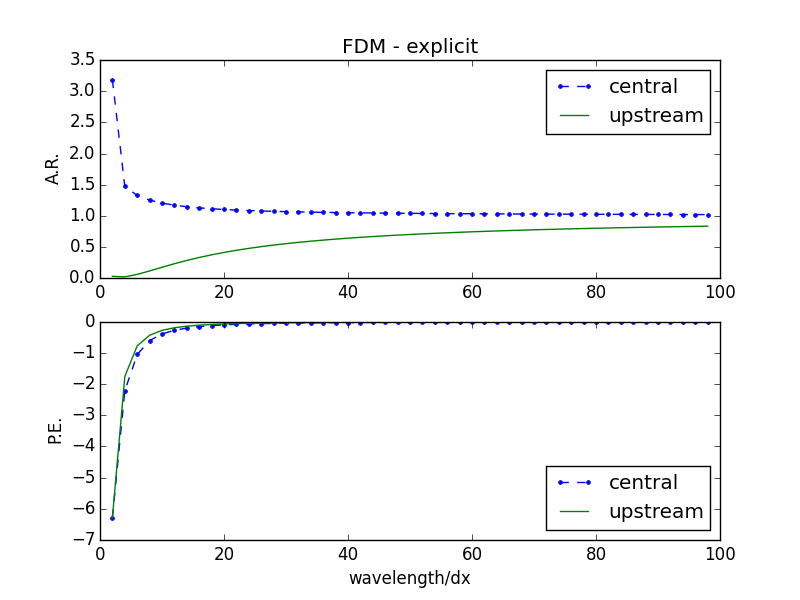
\includegraphics[scale=0.5]{../part1/FDM_explicit_AR_PE.png}
    }\qquad
    \subfloat[Crank-Nicolson]{
      \label{fig:1b}
      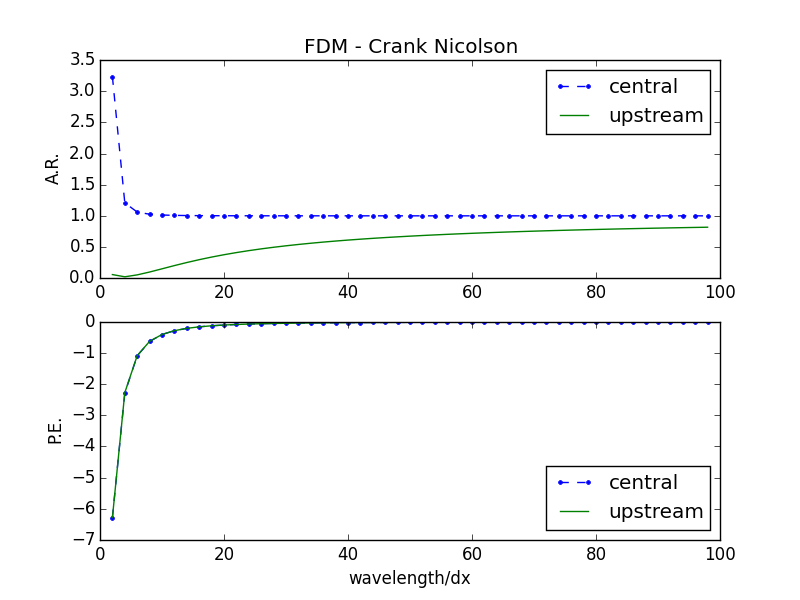
\includegraphics[scale=0.5]{../part1/FDM_CN_AR_PE.png}
    }%
    \caption{AR and PE plots of finite difference solutions.}
    \label{fig:1}
\end{figure}

\subsubsection{Numerical solutions versus analytical solutions}
\paragraph{Numerical solutions - upstream} The scheme of the numerical solutions to the upstream - explicit - finite difference method can be fomulated as follows.

\begin{equation}
  \label{eq:7}
  A_{fdm,explicit,up}{\tilde{c}}^{k+1}=B_{fdm,explicit,up}{\tilde{c}}^{k}+b_{fdm,explicit,up}
\end{equation}

in which

\begin{subequations}
  \begin{equation}
    A_{fdm,explicit,up} = I_{N\times N}
  \end{equation}
  \begin{equation}
    B_{fdm,explicit,up} = \begin{bmatrix}
      1-(\alpha +1)\mathcal{D}-\alpha\mathcal{U} & \mathcal{D} & 0 & 0 & \cdots & 0 \\
      \mathcal{D}+\mathcal{U} & -(2\mathcal{D}+\mathcal{U}-1) & \mathcal{D} & 0 & \cdots & 0 \\
      0 & \mathcal{D}+\mathcal{U} & -(2\mathcal{D}+\mathcal{U}-1) & \mathcal{D} & \cdots & 0\\
      \vdots & \vdots & \ddots & \ddots & \ddots & \vdots \\
      0 & 0 & \cdots & \mathcal{D}+\mathcal{U} & -(2\mathcal{D}+\mathcal{U}-1) & \mathcal{D} \\
      0 & 0 & \cdots & 0 & \mathcal{D}+\mathcal{U} & -(2\mathcal{D}+\mathcal{U}-1)
      \end{bmatrix}_{N\times N}
  \end{equation}
  \begin{equation}
    b_{fdm,explicit,up} = \{\alpha(\mathcal{D}+\mathcal{U})c_{Feed}, 0, \dots, 0\}_{1\times N}^T
  \end{equation}
\end{subequations}

where $\alpha=\frac{\Delta xu}{D}$.

\paragraph{Numerical solutions - central} The scheme of the numerical solutions to the central - finite difference method can be fomulated as follows.

\begin{equation}
  \label{eq:8}
  A_{fdm,explicit,central}{\tilde{c}}^{k+1}=B_{fdm,explicit,central}{\tilde{c}}^{k}+b_{fdm,explicit,central}
\end{equation}

in which

\begin{subequations}
  \begin{equation}
    A_{fdm,explicit,central} = I_{N\times N}
  \end{equation}
  \begin{equation}
    B_{fdm,explicit,central} = \begin{bmatrix}
      1-2(\alpha +1)\mathcal{D}-\alpha\mathcal{U} & 2\mathcal{D} & 0 & 0 & \cdots & 0 \\
      \mathcal{D}+\mathcal{U}/2 & 1-2\mathcal{D} & \mathcal{D}-\mathcal{U} & 0 & \cdots & 0 \\
      \vdots & \vdots & \ddots & \ddots & \ddots & \vdots \\
      0 & 0 & \cdots & \mathcal{D}+\mathcal{U}/2 & 1-2\mathcal{D} & \mathcal{D}-\mathcal{U} \\
      0 & 0 & \cdots & 0 & \mathcal{D}+\mathcal{U}/2 & 1-2\mathcal{D}
      \end{bmatrix}_{N\times N}
  \end{equation}
  \begin{equation}
    b_{fdm,explicit,central} = \{\alpha(\mathcal{D}+\mathcal{U})c_{Feed}, 0, \dots, 0\}_{1\times N}^T
  \end{equation}
\end{subequations}

where $\alpha=\frac{\Delta xu}{D}$.

\paragraph{Settings} The save as the settings in Section~\ref{partA-setting}.

\paragraph{Result} The numerial and analytical of solutions the two methods (i.e., upstream and central methods) by usnig explicit finite difference at T = 50 days and 100 days are plotted in Figure \ref{fig:2}. The values are shown in the Appendix.

\paragraph{Discussion}\label{fdm-explicit-discussion} Both the results simulated at T=50 and T=100 show that compared with the analytical solutions, the numerical results of the central methods generate oscillations while numerical dispersions occur in the upstream method. These results are compatible with the Fourier analysis of part (a). As shown in part (a), the A.R. values of the central method are around 3 for small wavelengths, causing the numerical oscillation behaviors shown in the figure. Also, the low A.R. values of the upstream method for small wavelengths result in the numerical dispersion of the numerical solutions.

\begin{figure}[!htbp]
    \centering
    \subfloat[50 days]{
      \label{fig:2a}
      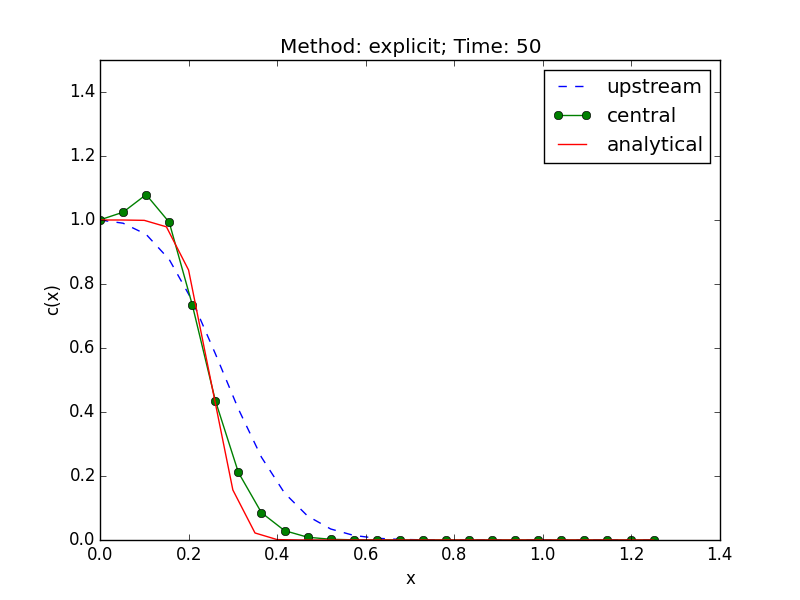
\includegraphics[scale=0.5]{../part1/explicit_50.png}
    }\qquad
    \subfloat[100 days]{
      \label{fig:2b}
      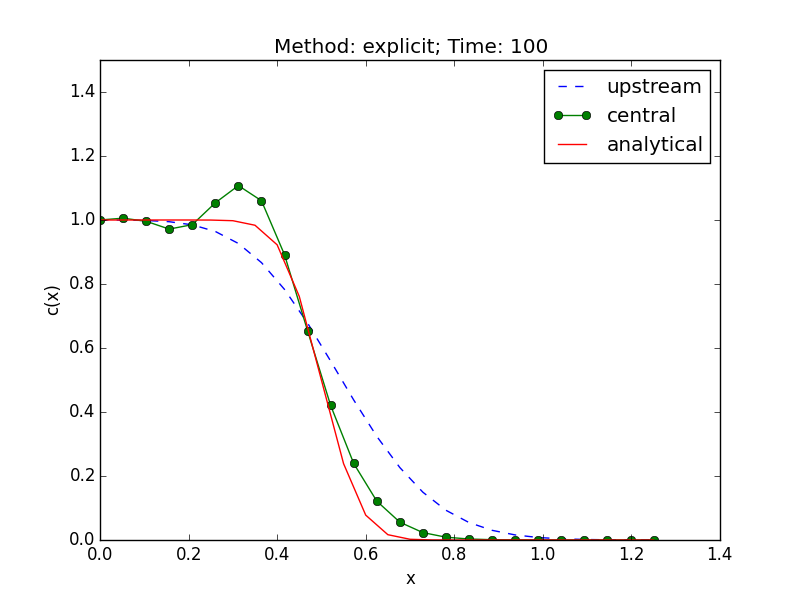
\includegraphics[scale=0.5]{../part1/explicit_100.png}
    }%
    \caption{Numerical and analytical solutions of explicit finite difference solutions at T = 50 days and 100 days.}
    \label{fig:2}
\end{figure}

\subsubsection{Stability examination with different $\Delta t$}
The stability condition of the explicit-upstream-finite difference method is
\begin{equation}
  \label{eq:stable}
  2\mathcal{D}+\mathcal{U} \leq 1
\end{equation}

We can get when $\Delta t \geq 8.33$, the numerical solution will be unstable.

\paragraph{Test 1} By assuming $\Delta t = 8.5$ days and the remaining setting remains unchanged, Figure~\ref{fig:3a} shows the numerical solutions at T = 8.5 days, 17 days, 25.5 days and 34 days. It can be seen from this figure that the numerical solution goes unstable very quickly.

\paragraph{Test 2} To further test the impact of $\Delta t$, we select $\Delta t = 2$ days. Figure~\ref{fig:3b} shows the numerical solutions at T = 2 days, 4 days, 6 days and 8 days. Similarly, it can be observed that the numerical solutions are unstable significantly.

\paragraph{Discussion} Through the two tests with $\Delta t = $ 8.5 days and 2 days, we conclude that the 3rd-type boundary condition would reduce the stability limit and enhance the unstable behavior with the increase of $\Delta t$. Even though in test 2, $\Delta t$ (2 days) is within the stable condition (Eq.~\ref{eq:stable}), the 3rd-type boundary condition still results in the unstable behavior of the numerical solutions.

\begin{figure}[!htbp]
    \centering
    \subfloat[Explicit]{
      \label{fig:3a}
      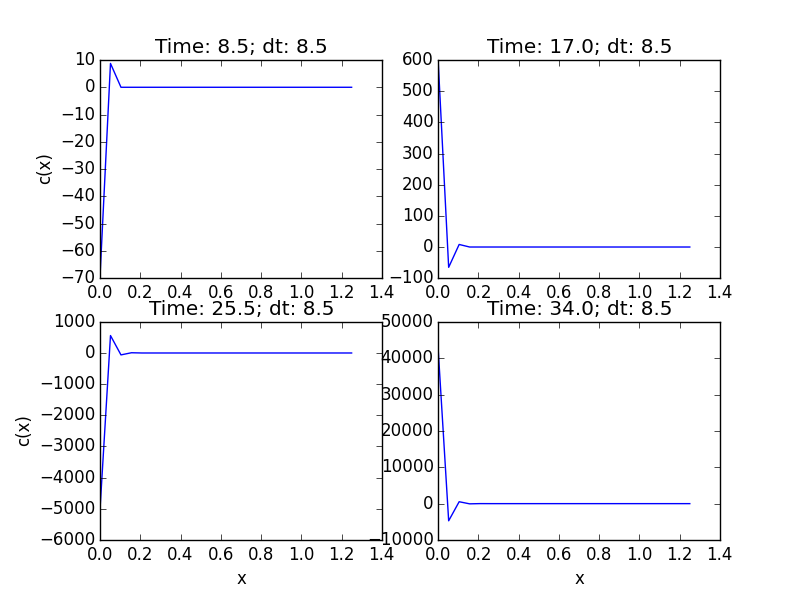
\includegraphics[scale=0.6]{../part1/stable_check_dt_85.png}
    }\qquad
    \subfloat[Crank-Nicolson]{
      \label{fig:3b}
      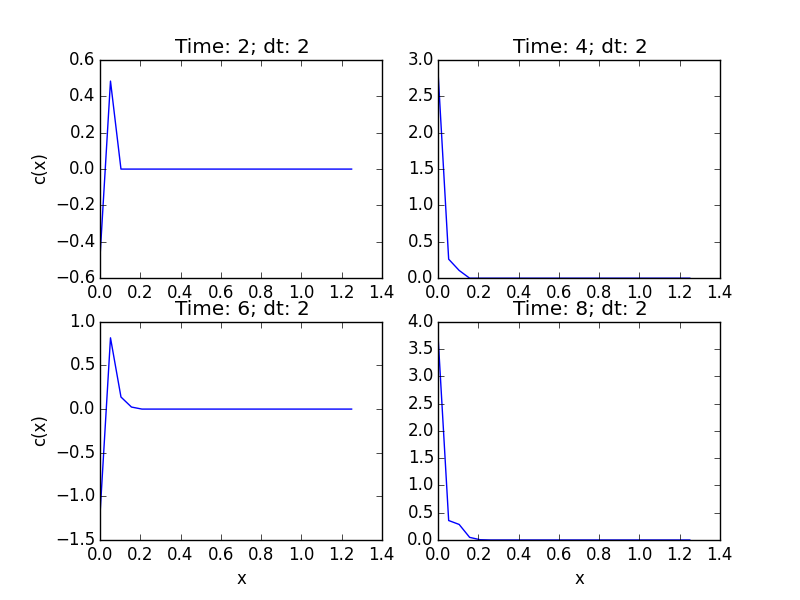
\includegraphics[scale=0.6]{../part1/stable_check_dt_2.png}
    }%
    \caption{AR and PE plots of finite difference solutions.}
    \label{fig:3}
\end{figure}

\subsection{Crank-Nicolson Solutions}
\subsubsection{AR and PE plots}
The numerical solutions of the amplification factor and phase shift of the upstream method are
\begin{subequations}
  \begin{equation}
    \label{eq:11a}
    \Phi_n^{fdm,CN,up} = \frac{1-(\mathcal{D}+\mathcal{U}/2)(1-\cos{2\pi \frac{\Delta x}{\Lambda_n}}) - i\frac{\mathcal{U}}{2}\sin{2\pi \frac{\Delta x}{\Lambda_n}}}{1-(\mathcal{D}+\mathcal{U}/2)(1-\cos{2\pi \frac{\Delta x}{\Lambda_n}}) + i\frac{\mathcal{U}}{2}\sin{2\pi \frac{\Delta x}{\Lambda_n}}}
  \end{equation}
  \begin{equation}
    \label{eq:11b}
    \Delta \Theta_n^{fdm,CN,up} = \sin^{-1}[\frac{-\mathcal{U}\sin{2\pi\frac{\Delta x}{\Lambda_n}}}{|\Phi_n^{fdm,CN,up}|}]
  \end{equation}
\end{subequations}

The numberical solutions of the amplification factor and phase shift of the central method are
\begin{subequations}
  \begin{equation}
    \label{eq:12a}
    \Phi_n^{fdm,CN,central} = \frac{1-\mathcal{D}(1-\cos{2\pi \frac{\Delta x}{\Lambda_n}}) - i\frac{\mathcal{U}}{2}\sin{2\pi \frac{\Delta x}{\Lambda_n}}}{1-\mathcal{D}(1-\cos{2\pi \frac{\Delta x}{\Lambda_n}}) + i\frac{\mathcal{U}}{2}\sin{2\pi \frac{\Delta x}{\Lambda_n}}}
  \end{equation}
  \begin{equation}
    \label{eq:12b}
    \Delta \Theta_n^{fdm,CN,central} = \sin^{-1}[\frac{-\mathcal{U}\sin{2\pi\frac{\Delta x}{\Lambda_n}}}{|\Phi_n^{fdm,CN,central}|}]
  \end{equation}
\end{subequations}

Therefore, the amplification ratios and the phase errors of the two methods can be obtained as follows.
\begin{subequations}
  \begin{equation}
    \label{eq:13a}
    AR_{fdm,CN,i} = (\frac{|\Phi_n^{fdm,CN,i}|}{|\Phi_n^{anal}|})^{Nn}
  \end{equation}
  \begin{equation}
    \label{eq:13b}
    PE_{fdm,CN,i} = -2\pi-Nn\Delta \Theta_n^{fdm,CN,i}
  \end{equation}
\end{subequations}
where $i=up,central$.

\paragraph{Settings} The save as the settings in Section~\ref{partA-setting}.

\paragraph{Result} The results of AR and PE of the two methods (i.e., upstream and central methods) by usnig explicit finite difference are plotted in Figure \ref{fig:1b}. The values are shown in the Appendix.

\paragraph{Discussion}  The A.R. and P.E. values of the Crank Nicolson method are almost
the same as that of the explicit method for the central and upstream
differences. Please refer to Section~\ref{partA1-ARPE-discussion} for details.

\subsubsection{Numerical solutions versus analytical solutions}
\paragraph{Numerical solutions - upstream} The scheme of the numerical solutions to the upstream - Crank Nicolson - finite difference method can be fomulated as follows.

\begin{equation}
  \label{eq:14}
  A_{D,fdm,CN,up}{\tilde{c}}^{k+1}+A_{A,fdm,CN,up}{\tilde{c}}^{k+1}=B_{D,fdm,CN,up}{\tilde{c}}^{k}+B_{A,fdm,CN,up}{\tilde{c}}^{k}+b_{fdm,CN,up}
\end{equation}

in which

\begin{subequations}
  \begin{equation}
    A_{D,fdm,CN,up} = \begin{bmatrix}
      (\alpha+1)\mathcal{D}/2+1 & -\mathcal{D}/2 & 0 & 0 & \cdots & 0 \\
      -\mathcal{D}/2 & \mathcal{D}+1 & -\mathcal{D}/2 & 0 & \cdots & 0 \\
      0 & -\mathcal{D}/2 & \mathcal{D}+1 & -\mathcal{D}/2 & \cdots & 0 \\
      \vdots & \vdots & \ddots & \ddots & \ddots & \vdots \\
      0 & 0 & \cdots & -\mathcal{D}/2 & \mathcal{D}+1 & -\mathcal{D}/2\\
      0 & 0 & 0 & \cdots & -\mathcal{D}/2 & \mathcal{D}+1
    \end{bmatrix}_{N\times N}
  \end{equation}
  \begin{equation}
    B_{D,fdm,explicit,up} = \begin{bmatrix}
      1-(\alpha+1)\mathcal{D}/2 & \mathcal{D}/2 & 0 & 0 & \cdots & 0 \\
      \mathcal{D}/2 & 1-\mathcal{D} & \mathcal{D}/2 & 0 & \cdots & 0 \\
      0 & \mathcal{D}/2 & 1-\mathcal{D} & \mathcal{D}/2 & \cdots & 0 \\
      \vdots & \vdots & \ddots & \ddots & \ddots & \vdots \\
      0 & 0 & \cdots & \mathcal{D}/2 & 1-\mathcal{D} & \mathcal{D}/2 \\
      0 & 0 & 0 & \cdots & \mathcal{D}/2 & 1-\mathcal{D}
      \end{bmatrix}_{N\times N}
  \end{equation}
  \begin{equation}
    A_{A,fdm,CN,up} = \begin{bmatrix}
      \alpha\mathcal{U}/2 & 0 & \cdots & 0 \\
      -\mathcal{U}/2 & \mathcal{U}/2 & \cdots & 0 \\
      \vdots & \ddots & \ddots  & \vdots \\
      0 & \cdots & -\mathcal{U}/2 & \mathcal{U}/2
    \end{bmatrix}_{N\times N}
  \end{equation}
  \begin{equation}
    B_{A,fdm,explicit,up} = \begin{bmatrix}
      -\alpha\mathcal{U}/2 & 0 & \cdots & 0 \\
      \mathcal{U}/2 & -\mathcal{U}/2 & \cdots & 0 \\
      \vdots & \ddots & \ddots  & \vdots \\
      0 & \cdots & \mathcal{U}/2 & -\mathcal{U}/2
      \end{bmatrix}_{N\times N}
  \end{equation}
  \begin{equation}
    b_{fdm,explicit,up} = \{\alpha(\mathcal{D}+\mathcal{U})c_{Feed}, 0, \dots, 0\}_{1\times N}^T
  \end{equation}
\end{subequations}

where $\alpha=\frac{\Delta xu}{D}$.

\paragraph{Numerical solutions - central} The scheme of the numerical solutions to the central - finite difference method can be fomulated as follows.

\begin{equation} A_{D,fdm,CN,central}{\tilde{c}}^{k+1}+A_{A,fdm,CN,central}{\tilde{c}}^{k+1}=B_{D,fdm,CN,central}{\tilde{c}}^{k}+B_{A,fdm,CN,central}{\tilde{c}}^{k}+b_{fdm,CN,central}
\end{equation}

in which

\begin{subequations}
  \begin{equation}
    A_{D,fdm,CN,central} = \begin{bmatrix}
      (\alpha+1)\mathcal{D}+1 & -\mathcal{D} & 0 & 0 & \cdots & 0 \\
      -\mathcal{D}/2 & \mathcal{D}+1 & -\mathcal{D}/2 & 0 & \cdots & 0 \\
      0 & -\mathcal{D}/2 & \mathcal{D}+1 & -\mathcal{D}/2 & \cdots & 0 \\
      \vdots & \vdots & \ddots & \ddots & \ddots & \vdots \\
      0 & 0 & \cdots & -\mathcal{D}/2 & \mathcal{D}+1 & -\mathcal{D}/2\\
      0 & 0 & 0 & \cdots & -\mathcal{D}/2 & \mathcal{D}+1
    \end{bmatrix}_{N\times N}
  \end{equation}
  \begin{equation}
    B_{D,fdm,explicit,central} = \begin{bmatrix}
      1-(\alpha+1)\mathcal{D} & \mathcal{D} & 0 & 0 & \cdots & 0 \\
      \mathcal{D}/2 & 1-\mathcal{D} & \mathcal{D}/2 & 0 & \cdots & 0 \\
      0 & \mathcal{D}/2 & 1-\mathcal{D} & \mathcal{D}/2 & \cdots & 0 \\
      \vdots & \vdots & \ddots & \ddots & \ddots & \vdots \\
      0 & 0 & \cdots & \mathcal{D}/2 & 1-\mathcal{D} & \mathcal{D}/2 \\
      0 & 0 & 0 & \cdots & \mathcal{D}/2 & 1-\mathcal{D}
      \end{bmatrix}_{N\times N}
  \end{equation}
  \begin{equation}
    A_{A,fdm,CN,central} = \begin{bmatrix}
      \alpha\mathcal{U}/2 & 0 & 0 & \cdots & 0 \\
      -\mathcal{U}/4 & 0 & \mathcal{U}/4 & \cdots & 0 \\
      \vdots & \ddots & \ddots & \ddots & \vdots \\
      0 & \cdots & -\mathcal{U}/4 & 0 & \mathcal{U}/4 \\
      0 & \cdots & 0 & -\mathcal{U}/4 & 0 \\
    \end{bmatrix}_{N\times N}
  \end{equation}
  \begin{equation}
    B_{A,fdm,explicit,central} = \begin{bmatrix}
      -\alpha\mathcal{U}/2 & 0 & 0 & \cdots & 0 \\
      \mathcal{U}/4 & 0 & -\mathcal{U}/4 & \cdots & 0 \\
      \vdots & \ddots & \ddots & \ddots & \vdots \\
      0 & \cdots & \mathcal{U}/4 & 0 & -\mathcal{U}/4 \\
      0 & \cdots & 0 & \mathcal{U}/4 & 0 \\
       \end{bmatrix}_{N\times N}
  \end{equation}
  \begin{equation}
    b_{fdm,explicit,central} = \{\alpha(2\mathcal{D}+\mathcal{U})c_{Feed}, 0, \dots, 0\}_{1\times N}^T
  \end{equation}
\end{subequations}

where $\alpha=\frac{\Delta xu}{D}$.

\paragraph{Settings} The save as the settings in Section~\ref{partA-setting}.

\paragraph{Result} The numerial and analytical of solutions the two methods (i.e., upstream and central methods) by usnig Crank-Nicolson finite difference at T = 50 days and 100 days are plotted in Figure \ref{fig:4}. The values are shown in the Appendix.

\paragraph{Discussion} Similar to the comparisons of the explicit method discussed in part 1(b), for Crank Nicolson method, the upstream difference causes numerical dispersions and the central difference induces numerical oscillations. It complies with the Fourier analysis shown in part 2(a), as discussed in Section~\ref{fdm-explicit-discussion}.

\begin{figure}[!htbp]
    \centering
    \subfloat[50 days]{
      \label{fig:4a}
      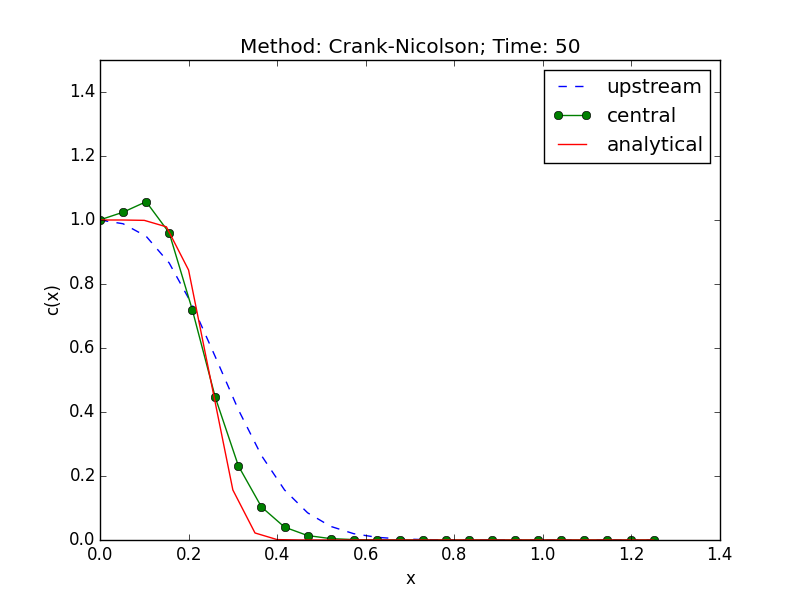
\includegraphics[scale=0.5]{../part1/Crank-Nicolson_50.png}
    }\qquad
    \subfloat[100 days]{
      \label{fig:4b}
      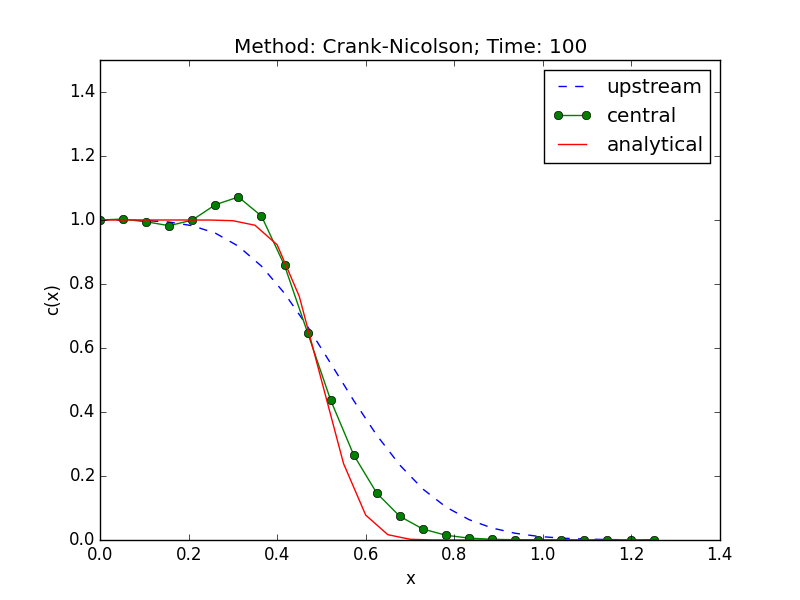
\includegraphics[scale=0.5]{../part1/Crank-Nicolson_100.png}
    }%
    \caption{Numerical and analytical solutions of Crank-Nicolson finite difference solutions at T = 50 days and 100 days.}
    \label{fig:4}
\end{figure}

\subsection{Mass Balance Analysis}
\paragraph{Analytical solution} The total mass of the analytical solution at time T is calculated as follows.
\begin{equation}
  m_{anal,T}=c_{feed}\times u \times T
\end{equation}

\paragraph{Numerical solution} The total mass of the numerical solution at time T is calculated as follows
\begin{equation}
  m_{fdm,i,j}^T = \sum\limits_{i=1}^{N-1} \frac{\tilde{c_i^T} + \tilde{c_{i+1}^T}}{2}\times \Delta x
\end{equation}
where $i$ is explicit or central and $j$ is up or central.

\paragraph{Result \& Discussion} The results of the mass of both the analytical and numerical solutions at T = 50 days and 100 days are shown in the Table~\ref{table:mass}. It can be seen from the table that in terms of the total mass, the solutions by using the central method outperform that using the upstream method. This is probably because despite the numerical oscillation generated by the central method, the central method is able to keep the total mass while the upstream method would result in a larger total mass because of the numerical dispersion. Meanwhile, Crank-Nicolson and the explicit method provide almost identical mass at a specific time.
\begin{table}[ht]
\caption{Nonlinear Model Results}
\centering
\begin{tabular}{c c c c c c}
\hline\hline 
time & analytical & explicit-up & explicit-central & CN-up & CN-central \\ [0.5ex]
\hline
50 &  0.25000 & 0.27993 & 0.25526 & 0.27992 & 0.25509 \\ 
100 & 0.50000 & 0.52999 & 0.50492 & 0.52998 & 0.50493 \\ [1ex]
\hline
\end{tabular}
\label{table:mass}
\end{table}
%%% Local Variables:
%%% mode: latex
%%% TeX-master: t
%%% End:
